\documentclass[11pt,a4paper]{article}
\usepackage[T1]{fontenc}
\usepackage[utf8]{inputenc}
\usepackage[provide=*,italian]{babel}
\usepackage{lmodern,microtype}
\usepackage{geometry}
\geometry{margin=2.5cm}
\usepackage{amsmath,amssymb,amsthm,mathtools}
\usepackage{booktabs,array,longtable,blkarray}
\usepackage{xcolor,enumitem}
\usepackage{tikz}
\usetikzlibrary{arrows.meta,positioning,calc}
\usepackage[most]{tcolorbox}
\usepackage{listings}
\usepackage{hyperref,fancyhdr}

\definecolor{sapienzared}{RGB}{130,0,36}
\definecolor{softred}{RGB}{249,241,243}
\definecolor{softblue}{RGB}{239,246,252}
\definecolor{softgray}{RGB}{245,245,245}
\definecolor{codegreen}{RGB}{25,110,65}
\hypersetup{colorlinks=true,linkcolor=sapienzared,urlcolor=sapienzared,
pdftitle={Grafi orientati e non orientati},pdfauthor={Giampaolo Liuzzi}}

\pagestyle{fancy}
\fancyhf{}
\fancyhead[L]{\small Ottimizzazione su Reti}
\fancyhead[R]{\small Capitolo 2}
\fancyfoot[C]{\thepage}
\renewcommand{\headrulewidth}{0.4pt}

\newtheorem{definition}{Definizione}[section]
\newtheorem{theorem}[definition]{Teorema}
\newtheorem{proposition}[definition]{Proposizione}
\newtheorem{observation}[definition]{Osservazione}

\newtcolorbox{learningbox}{colback=softred,colframe=sapienzared,
title=Obiettivi di apprendimento,fonttitle=\bfseries,boxrule=0.8pt,arc=1.5mm}
\newtcolorbox{examplebox}[1]{colback=softblue,colframe=blue!55!black,
title=#1,fonttitle=\bfseries,boxrule=0.7pt,arc=1.5mm}
\newtcolorbox{notationbox}{colback=softgray,colframe=black!55,
title=Registro delle notazioni,fonttitle=\bfseries,boxrule=0.7pt,arc=1.5mm}
\newtcolorbox{warningbox}{colback=yellow!9,colframe=orange!65!black,
title=Attenzione,fonttitle=\bfseries,boxrule=0.7pt,arc=1.5mm}
\newtcolorbox{networkxbox}{colback=softgray,colframe=black!55,
title=Python/NetworkX,fonttitle=\bfseries,boxrule=0.7pt,arc=1.5mm}

\lstdefinestyle{python}{language=Python,basicstyle=\ttfamily\small,
keywordstyle=\color{blue!65!black}\bfseries,commentstyle=\color{codegreen},
stringstyle=\color{sapienzared},backgroundcolor=\color{softgray},frame=single,
rulecolor=\color{black!25},showstringspaces=false,breaklines=true,columns=fullflexible}

\newcommand{\V}{\mathcal{V}}
\newcommand{\E}{\mathcal{E}}
\newcommand{\N}{\mathcal{N}}
\newcommand{\R}{\mathbb{R}}
\newcommand{\deltaout}{\delta^{+}}
\newcommand{\deltain}{\delta^{-}}

\begin{document}
\hypersetup{pageanchor=false}
\begin{titlepage}
\centering
\vspace*{1.6cm}
{\color{sapienzared}\rule{\textwidth}{1.2pt}}\\[1.1cm]
{\Large Ottimizzazione su Reti}\\[0.35cm]
{\huge\bfseries Capitolo 2}\\[0.45cm]
{\LARGE\bfseries Grafi orientati e non orientati}\\[1.1cm]
{\color{sapienzared}\rule{0.72\textwidth}{0.8pt}}\\[1.1cm]
{\large Corso di Laurea Magistrale in Ingegneria Gestionale}\\[0.25cm]
{\large Sapienza Università di Roma}\\[1.2cm]
{\large Giampaolo Liuzzi}\\[0.25cm]
{\normalsize Dipartimento di Ingegneria Informatica, Automatica e Gestionale}\\[2cm]
\vfill
{\small Versione preliminare per uso didattico}
\end{titlepage}
\hypersetup{pageanchor=true}
\pagenumbering{roman}
\tableofcontents
\newpage
\pagenumbering{arabic}

\begin{learningbox}
Al termine del capitolo lo studente dovrebbe essere in grado di:
\begin{itemize}[nosep]
\item definire grafi orientati e non orientati e riconoscerne gli elementi;
\item usare correttamente adiacenza, incidenza, intorni e gradi;
\item distinguere passeggiate, cammini, circuiti e cicli;
\item costruire sottografi e sottografi indotti;
\item determinare componenti connesse e fortemente connesse;
\item rappresentare un grafo mediante liste, matrici e NetworkX;
\item scegliere la rappresentazione più adatta a uno specifico algoritmo.
\end{itemize}
\end{learningbox}

\section{Grafi non orientati}

\begin{definition}[Grafo non orientato]
Un grafo non orientato è una coppia
\[
G=(\V,\E),
\]
dove $\V$ è un insieme finito di \emph{nodi} o \emph{vertici} ed $\E$ è un insieme di coppie non ordinate di nodi, dette \emph{spigoli}.
\end{definition}

Per distinguere chiaramente gli spigoli dagli archi orientati, scriveremo uno spigolo tra $i$ e $j$ come $\{i,j\}$. Poiché la coppia non è ordinata,
\[
\{i,j\}=\{j,i\}.
\]
Poniamo $n=|\V|$ e $m=|\E|$.

\begin{examplebox}{Confini geografici}
Se i nodi rappresentano regioni e gli spigoli rappresentano confini comuni, la relazione è simmetrica: se $i$ confina con $j$, allora $j$ confina con $i$. Il modello naturale è quindi un grafo non orientato.
\end{examplebox}

\section{Grafi orientati}

\begin{definition}[Grafo orientato]
Un grafo orientato, o digrafo, è una coppia $G=(\V,\E)$ nella quale $\V$ è l'insieme dei nodi ed $\E\subseteq\V\times\V$ è un insieme di coppie ordinate, dette \emph{archi}.
\end{definition}

L'arco $(i,j)$ ha origine, o coda, nel nodo $i$ e destinazione, o testa, nel nodo $j$. In generale $(i,j)$ e $(j,i)$ sono archi distinti e possono esistere indipendentemente.

\begin{figure}[ht]
\centering
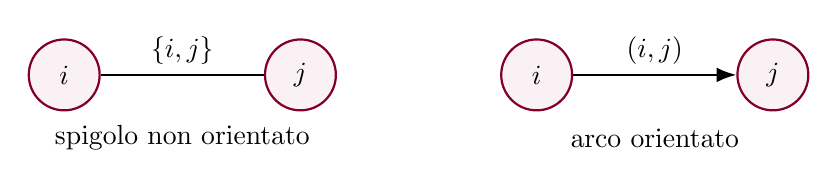
\begin{tikzpicture}[
node/.style={circle,draw=sapienzared,thick,fill=softred,minimum size=9mm},
edge/.style={thick},arc/.style={-{Latex[length=2.5mm]},thick}]
\node[node] (a) at (0,0) {$i$};
\node[node] (b) at (3,0) {$j$};
\draw[edge] (a) -- node[above] {$\{i,j\}$} (b);
\node at (1.5,-0.8) {spigolo non orientato};
\node[node] (c) at (6,0) {$i$};
\node[node] (d) at (9,0) {$j$};
\draw[arc] (c) -- node[above] {$(i,j)$} (d);
\node at (7.5,-0.8) {arco orientato};
\end{tikzpicture}
\caption{Spigolo e arco: l'orientamento fa parte del dato.}
\end{figure}

Esempi naturalmente orientati sono i collegamenti a senso unico, i link tra pagine web e le relazioni di precedenza tra attività.

\subsection{Grafi semplici, cappi e archi multipli}

\begin{definition}[Grafo semplice]
Un grafo è semplice se non contiene cappi, cioè collegamenti di un nodo con se stesso, e non contiene collegamenti multipli tra la stessa coppia di nodi.
\end{definition}

Nelle presenti dispense, salvo indicazione contraria, i grafi saranno semplici. Quando occorrerà rappresentare più collegamenti paralleli useremo esplicitamente un multigrafo.

\section{Adiacenza, incidenza, intorni e gradi}

\subsection{Grafo non orientato}

Due nodi $i$ e $j$ sono \emph{adiacenti} se $\{i,j\}\in\E$. Uno spigolo è \emph{incidente} sui suoi due estremi. L'intorno di $i$ è
\[
\N(i)=\{j\in\V:\{i,j\}\in\E\}.
\]
La stella di $i$ è l'insieme degli spigoli incidenti su $i$:
\[
\delta(i)=\{e\in\E:i\in e\}.
\]
Il grado di $i$ è
\[
\deg(i)=|\delta(i)|=|\N(i)|
\]
per un grafo semplice.

\begin{proposition}[Lemma della stretta di mano]
Per ogni grafo non orientato,
\[
\sum_{i\in\V}\deg(i)=2|\E|.
\]
\end{proposition}
Ogni spigolo contribuisce infatti una unità al grado di ciascuno dei suoi due estremi.

\subsection{Grafo orientato}

Per un nodo $i$ definiamo l'intorno uscente e quello entrante:
\begin{align*}
\N^+(i)&=\{j\in\V:(i,j)\in\E\},\\
\N^-(i)&=\{j\in\V:(j,i)\in\E\}.
\end{align*}
Analogamente, le stelle uscente ed entrante sono
\begin{align*}
\deltaout(i)&=\{(i,j)\in\E\},\\
\deltain(i)&=\{(j,i)\in\E\}.
\end{align*}
Il grado uscente e il grado entrante sono
\[
\deg^+(i)=|\deltaout(i)|,
\qquad
\deg^-(i)=|\deltain(i)|.
\]
Vale
\[
\sum_{i\in\V}\deg^+(i)=\sum_{i\in\V}\deg^-(i)=|\E|.
\]

\begin{warningbox}
Nei grafi orientati il termine ``adiacente'' può essere ambiguo se non si specifica la direzione. Useremo preferibilmente ``successore'' per un nodo in $\N^+(i)$ e ``predecessore'' per un nodo in $\N^-(i)$.
\end{warningbox}

\section{Sottografi}

\begin{definition}[Sottografo]
Sia $G=(\V,\E)$. Un grafo $H=(W,F)$ è un sottografo di $G$ se
\[
W\subseteq\V,\qquad F\subseteq\E,
\]
e ogni collegamento in $F$ ha entrambi gli estremi in $W$.
\end{definition}

\begin{definition}[Sottografo indotto]
Dato $W\subseteq\V$, il sottografo indotto da $W$, indicato con $G[W]$, contiene tutti e soli i collegamenti di $G$ aventi entrambi gli estremi in $W$.
\end{definition}

Un sottografo generico può omettere collegamenti tra nodi che conserva; un sottografo indotto non può farlo.

\begin{examplebox}{Stessi nodi e spigoli diversi}
Consideriamo il grafo non orientato
\[
\V=\{1,2,3,4\},\qquad
\E=\bigl\{\{1,2\},\{1,3\},\{2,3\},\{2,4\},\{3,4\}\bigr\}
\]
e scegliamo il sottoinsieme di nodi $W=\{1,2,3\}$.

Il grafo $H=(W,F)$ con
\[
F=\bigl\{\{1,2\},\{2,3\}\bigr\}
\]
è un sottografo di $G$: conserva i nodi 1, 2 e 3, ma sceglie di omettere lo spigolo $\{1,3\}$. Il sottografo indotto $G[W]$, invece, deve conservare \emph{tutti} gli spigoli di $G$ i cui estremi appartengono a $W$; contiene quindi anche $\{1,3\}$.

\begin{center}
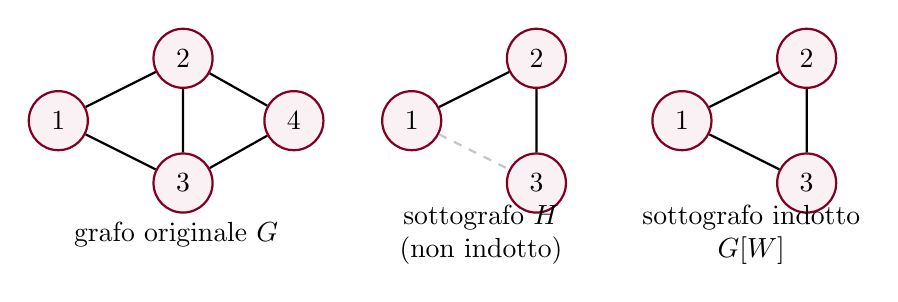
\begin{tikzpicture}[
node/.style={circle,draw=sapienzared,thick,fill=softred,minimum size=7.5mm},
edge/.style={thick},faded/.style={black!22,thick},scale=0.88]
% Grafo originale
\begin{scope}[xshift=0cm]
\node[node] (g1) at (0,1.5) {$1$};
\node[node] (g2) at (1.8,2.4) {$2$};
\node[node] (g3) at (1.8,0.6) {$3$};
\node[node] (g4) at (3.4,1.5) {$4$};
\draw[edge] (g1)--(g2)--(g3)--(g1);
\draw[edge] (g2)--(g4)--(g3);
\node at (1.7,-0.15) {grafo originale $G$};
\end{scope}
% Sottografo non indotto
\begin{scope}[xshift=5.1cm]
\node[node] (h1) at (0,1.5) {$1$};
\node[node] (h2) at (1.8,2.4) {$2$};
\node[node] (h3) at (1.8,0.6) {$3$};
\draw[edge] (h1)--(h2)--(h3);
\draw[faded,dashed] (h1)--(h3);
\node[align=center] at (1.0,-0.15) {sottografo $H$\\(non indotto)};
\end{scope}
% Sottografo indotto
\begin{scope}[xshift=9.0cm]
\node[node] (i1) at (0,1.5) {$1$};
\node[node] (i2) at (1.8,2.4) {$2$};
\node[node] (i3) at (1.8,0.6) {$3$};
\draw[edge] (i1)--(i2)--(i3)--(i1);
\node[align=center] at (1.0,-0.15) {sottografo indotto\\$G[W]$};
\end{scope}
\end{tikzpicture}
\end{center}

Nel disegno centrale lo spigolo tratteggiato indica il collegamento presente in $G$ ma deliberatamente escluso da $H$. Nel disegno a destra tale esclusione non è consentita: una volta scelto $W$, l'insieme degli spigoli di $G[W]$ è determinato automaticamente.
\end{examplebox}

In sintesi, per costruire un sottografo si scelgono nodi \emph{e} collegamenti; per costruire un sottografo indotto si scelgono soltanto i nodi.

\begin{definition}[Grafo parziale]
Un sottografo $H=(\V,F)$ che conserva tutti i nodi di $G$ è detto grafo parziale, o sottografo ricoprente.
\end{definition}

Questa nozione sarà importante quando studieremo alberi ricoprenti e basi del simplesso su reti.

\section{Passeggiate, cammini, circuiti e cicli}

Per evitare ambiguità terminologiche adottiamo le definizioni seguenti.

\begin{definition}[Passeggiata]
Una passeggiata da $v_0$ a $v_k$ è una sequenza
\[
v_0,e_1,v_1,e_2,\ldots,e_k,v_k
\]
nella quale ogni collegamento $e_r$ unisce $v_{r-1}$ e $v_r$. Nodi e collegamenti possono ripetersi.
\end{definition}

\begin{definition}[Cammino]
Un cammino è una passeggiata nella quale tutti i nodi sono distinti. Di conseguenza anche i collegamenti sono distinti.
\end{definition}

La lunghezza di una passeggiata o di un cammino è il numero dei collegamenti attraversati. Se ai collegamenti sono associati costi, il costo è la somma dei costi lungo la sequenza.

\begin{definition}[Circuito e ciclo]
Una passeggiata chiusa, cioè con $v_0=v_k$, è detta circuito. Un ciclo è un circuito nel quale $v_0,\ldots,v_{k-1}$ sono distinti.
\end{definition}

Nei grafi orientati distinguiamo inoltre il rispetto della direzione.

\begin{definition}[Cammino orientato]
In un digrafo, un cammino orientato da $v_0$ a $v_k$ è una sequenza di nodi distinti
\[
v_0,v_1,\ldots,v_k
\]
tale che $(v_{r-1},v_r)\in\E$ per ogni $r=1,\ldots,k$.
\end{definition}

Un ciclo orientato è un ciclo che percorre tutti gli archi secondo il loro orientamento.

\begin{observation}
Se esiste una passeggiata da $u$ a $v$, esiste anche un cammino da $u$ a $v$: è sufficiente eliminare successivamente le porzioni comprese tra due occorrenze dello stesso nodo.
\end{observation}

\begin{examplebox}{Orientamento e raggiungibilità}
Se esistono gli archi $(1,2)$ e $(2,3)$, allora $1,2,3$ è un cammino orientato da 1 a 3. Non segue che esista un cammino orientato da 3 a 1. Ignorando l'orientamento, invece, 1 e 3 appartengono alla stessa componente connessa.
\end{examplebox}

\section{Connessione}

\subsection{Grafi non orientati}

Due nodi $u$ e $v$ sono connessi se esiste un cammino tra essi. La relazione è riflessiva, simmetrica e transitiva; è quindi una relazione di equivalenza su $\V$.

\begin{definition}[Componente connessa]
Una componente connessa è il sottografo indotto da una classe di equivalenza della relazione di connessione. Un grafo è connesso se possiede una sola componente connessa.
\end{definition}

\subsection{Grafi orientati: connessione debole e forte}

Un digrafo è \emph{debolmente connesso} se il grafo non orientato ottenuto dimenticando la direzione degli archi è connesso.

\begin{definition}[Forte connessione]
Due nodi $u$ e $v$ sono fortemente connessi se esiste un cammino orientato da $u$ a $v$ e un cammino orientato da $v$ a $u$.
\end{definition}

La forte connessione è una relazione di equivalenza.

\begin{definition}[Componente fortemente connessa]
Una componente fortemente connessa è il sottografo indotto da una classe di equivalenza della forte connessione. Un digrafo è fortemente connesso se ha una sola componente fortemente connessa.
\end{definition}

Un digrafo fortemente connesso è anche debolmente connesso; il viceversa non è vero.

\section{Tagli}

Sia $S$ un sottoinsieme non vuoto e proprio di $\V$ e sia $\bar S=\V\setminus S$.

Per un grafo non orientato, il taglio associato a $S$ è
\[
\delta(S)=\{\{i,j\}\in\E:i\in S,\ j\in\bar S\}.
\]
Per un digrafo distinguiamo
\begin{align*}
\deltaout(S)&=\{(i,j)\in\E:i\in S,\ j\in\bar S\},\\
\deltain(S)&=\{(i,j)\in\E:i\in\bar S,\ j\in S\}.
\end{align*}

\begin{proposition}
Un grafo non orientato è non connesso se e solo se esiste un insieme non vuoto e proprio $S\subset\V$ tale che $\delta(S)=\varnothing$.
\end{proposition}

I tagli torneranno nello studio del massimo flusso, del minimo taglio e degli alberi ricoprenti.

\section{Rappresentazioni di un grafo}

Una stessa struttura può essere memorizzata in modi differenti. La scelta influenza memoria, facilità di accesso e complessità degli algoritmi.

\subsection{Rappresentazione estensiva}

La forma più diretta consiste nell'elencare $\V$ ed $\E$. È adatta a esempi piccoli e costituisce la base della lista degli archi.

\subsection{Matrice di adiacenza}

Per non confonderla con la matrice di incidenza $A$ del Capitolo 4, indichiamo la matrice di adiacenza con $M_G\in\{0,1\}^{n\times n}$:
\[
(M_G)_{ij}=\begin{cases}
1,&\text{se $(i,j)\in\E$ in un digrafo,}\cr
1,&\text{se $\{i,j\}\in\E$ in un grafo non orientato,}\cr
0,&\text{altrimenti.}
\end{cases}
\]
Per un grafo non orientato $M_G$ è simmetrica. La matrice richiede memoria $\Theta(n^2)$, indipendentemente dal numero di collegamenti.

\subsection{Liste di adiacenza}

A ogni nodo si associa la lista dei suoi vicini. Nei digrafi si usa normalmente la lista dei successori e, quando necessario, quella dei predecessori. La memoria richiesta è $\Theta(n+m)$ ed è quindi vantaggiosa per grafi sparsi.

\subsection{Matrice di incidenza}

La matrice di incidenza nodo-collegamento ha una riga per nodo e una colonna per spigolo o arco. Per un digrafo adotteremo la convenzione già fissata:
\[
a_{ve}=\begin{cases}
-1,&\text{se l'arco $e$ esce da $v$},\\
+1,&\text{se l'arco $e$ entra in $v$},\\
0,&\text{altrimenti.}
\end{cases}
\]
La matrice sarà studiata in dettaglio nel Capitolo 4.

\subsection{Confronto}

\begin{center}
\begin{tabular}{p{3.4cm}p{3.2cm}p{3.2cm}p{3.2cm}}
\toprule
Rappresentazione & Memoria & Vantaggio & Uso tipico\\
\midrule
Lista degli archi & $\Theta(m)$ & scansione semplice & input, ordinamento archi\\
Matrice di adiacenza & $\Theta(n^2)$ & test di adiacenza immediato & grafi densi\\
Liste di adiacenza & $\Theta(n+m)$ & visita dei vicini & grafi sparsi, percorsi\\
Matrice di incidenza & $\Theta(nm)$ in forma densa & struttura algebrica & flussi, modelli lineari\\
\bottomrule
\end{tabular}
\end{center}

\section{Grafi con NetworkX}

\begin{networkxbox}
NetworkX utilizza \texttt{Graph} per grafi non orientati e \texttt{DiGraph} per grafi orientati. Nodi e collegamenti possono possedere attributi; l'ordine di inserimento non deve essere confuso con una proprietà matematica del grafo.
\end{networkxbox}

\begin{lstlisting}[style=python,caption={Creazione di grafi e interrogazione della struttura.}]
import networkx as nx

# Grafo non orientato
H = nx.Graph()
H.add_nodes_from([1, 2, 3, 4])
H.add_edges_from([(1, 2), (1, 3), (2, 4), (3, 4)])

print(list(H.neighbors(1)))
print(H.degree[1])
print(list(nx.connected_components(H)))

# Grafo orientato
G = nx.DiGraph()
G.add_edges_from([(1, 2), (2, 3), (3, 2), (3, 4)])

print(list(G.successors(2)))
print(list(G.predecessors(2)))
print(G.out_degree[2], G.in_degree[2])
print(list(nx.strongly_connected_components(G)))
\end{lstlisting}

Le principali corrispondenze sono:
\begin{center}
\begin{tabular}{ll}
\toprule
Concetto & NetworkX\\
\midrule
intorno in un grafo non orientato & \texttt{G.neighbors(i)}\\
successori e predecessori & \texttt{G.successors(i)}, \texttt{G.predecessors(i)}\\
grado entrante e uscente & \texttt{G.in\_degree[i]}, \texttt{G.out\_degree[i]}\\
sottografo indotto & \texttt{G.subgraph(W)}\\
componenti connesse & \texttt{nx.connected\_components(G)}\\
componenti fortemente connesse & \texttt{nx.strongly\_connected\_components(G)}\\
matrice di adiacenza & \texttt{nx.adjacency\_matrix(G)}\\
matrice di incidenza orientata & \texttt{nx.incidence\_matrix(G, oriented=True)}\\
\bottomrule
\end{tabular}
\end{center}

\begin{warningbox}
Quando si confrontano matrici costruite manualmente e matrici prodotte da una libreria, occorre controllare l'ordine di nodi e archi e la convenzione dei segni. La struttura matematica può essere la stessa anche se righe o colonne compaiono in ordine diverso.
\end{warningbox}

\section{Registro delle notazioni aggiornato}

\begin{notationbox}
\begin{center}
\begin{tabular}{>{$}l<{$}p{10.0cm}}
\toprule
G=(\V,\E) & grafo con nodi $\V$ e collegamenti $\E$;\\
\{i,j\} & spigolo non orientato tra $i$ e $j$;\\
(i,j) & arco orientato da $i$ a $j$;\\
n=|\V|,\ m=|\E| & numero di nodi e collegamenti;\\
\N(i) & intorno di $i$ in un grafo non orientato;\\
\N^+(i),\ \N^-(i) & successori e predecessori di $i$;\\
\delta(i) & stella di $i$ in un grafo non orientato;\\
\deltaout(i),\ \deltain(i) & archi uscenti ed entranti in $i$;\\
\deg(i),\ \deg^+(i),\ \deg^-(i) & grado, grado uscente e grado entrante;\\
G[W] & sottografo indotto dal sottoinsieme di nodi $W$;\\
\delta(S),\ \deltaout(S),\ \deltain(S) & taglio non orientato, uscente ed entrante;\\
M_G & matrice di adiacenza;\\
A & matrice di incidenza nodo-arco.\\
\bottomrule
\end{tabular}
\end{center}
\end{notationbox}

\section{Errori frequenti}

\begin{enumerate}
\item Confondere lo spigolo $\{i,j\}$ con l'arco $(i,j)$.
\item Supporre che $(i,j)\in\E$ implichi $(j,i)\in\E$ in un digrafo.
\item Confondere un sottografo con il sottografo indotto dagli stessi nodi.
\item Chiamare ciclo una passeggiata chiusa che ripete nodi intermedi.
\item Usare la connessione debole quando l'algoritmo richiede raggiungibilità orientata.
\item Usare la stessa lettera per matrice di adiacenza e matrice di incidenza senza precisarlo.
\item Confrontare matrici senza controllare l'ordine di nodi e archi.
\end{enumerate}

\section{Esercizi}

\subsection*{Esercizio 2.1 - Concetti fondamentali}
Sia $G=(\V,\E)$ il digrafo con
\[
\V=\{1,2,3,4,5\},\quad
\E=\{(1,2),(1,3),(2,3),(3,2),(3,4),(4,5)\}.
\]
Determinare per ogni nodo successori, predecessori, grado uscente e grado entrante.

\subsection*{Esercizio 2.2 - Cammini e cicli}
Per il digrafo dell'Esercizio 2.1:
\begin{enumerate}[label=(\alph*)]
\item elencare due cammini orientati con origine 1;
\item individuare tutti i cicli orientati semplici;
\item stabilire quali nodi sono raggiungibili da 2;
\item stabilire se esiste un cammino orientato da 5 a 1.
\end{enumerate}

\subsection*{Esercizio 2.3 - Sottografi}
Costruire il sottografo indotto da $W=\{1,2,3,5\}$ e un sottografo non indotto avente lo stesso insieme di nodi. Spiegare la differenza.

\subsection*{Esercizio 2.4 - Connessione}
Determinare le componenti debolmente connesse e fortemente connesse del digrafo dell'Esercizio 2.1. Costruire poi un arco aggiuntivo che renda il grafo fortemente connesso, oppure spiegare perché un solo arco non è sufficiente.

\subsection*{Esercizio 2.5 - Rappresentazioni}
Per il digrafo dell'Esercizio 2.1, fissando l'ordine naturale dei nodi e l'ordine degli archi indicato:
\begin{enumerate}[label=(\alph*)]
\item costruire la matrice di adiacenza $M_G$;
\item scrivere le liste dei successori;
\item costruire la matrice di incidenza $A$ con $-1$ all'origine e $+1$ alla destinazione;
\item verificare che la somma degli elementi di ciascuna colonna di $A$ sia zero.
\end{enumerate}

\subsection*{Esercizio 2.6 - NetworkX}
Rappresentare il digrafo dell'Esercizio 2.1 con NetworkX e verificare automaticamente le risposte degli Esercizi 2.1--2.5. Rendere esplicito l'ordine di nodi e archi usato per produrre le matrici.

\section{Sintesi del capitolo}

\begin{tcolorbox}[colback=softred,colframe=sapienzared,boxrule=0.8pt,arc=1.5mm]
\begin{itemize}[nosep]
\item Un grafo non orientato usa spigoli $\{i,j\}$; un digrafo usa archi $(i,j)$.
\item Intorni, stelle e gradi descrivono la struttura locale di un nodo.
\item Sottografi indotti, cammini e cicli consentono di analizzare porzioni e percorsi del grafo.
\item La connessione nei grafi non orientati e la forte connessione nei digrafi sono relazioni di equivalenza.
\item Matrici e liste rappresentano la stessa struttura con costi computazionali differenti.
\item La matrice di adiacenza è indicata con $M_G$; $A$ è riservata alla matrice di incidenza.
\item In NetworkX occorre scegliere correttamente tra \texttt{Graph} e \texttt{DiGraph}.
\end{itemize}
\end{tcolorbox}

\section*{Verso il capitolo successivo}
Il Capitolo 3 studierà alberi, foreste, alberi ricoprenti e grafi orientati aciclici. Queste strutture saranno usate sia nelle basi del simplesso su reti sia negli algoritmi per cammini minimi e nella pianificazione di progetti.

\end{document}
